\addcontentsline{toc}{subsection}{Average Value \& Mean Value Theorem}
\subsection*{AVT \& MVT}
\begin{tcolorbox}[title= AVERAGE VALUE OF A FUNCTION,colframe=black,sharp corners,colback=white,colbacktitle=white,coltitle=black,boxrule=1pt]

     If $f$ is integrable on $[a,\,b]$, its average (mean) value on $[a,\,b]$ is
     \[\text{ave}(f)=\frac{1}{b-a}\int_a^b f(x)\,dx.\]
    
\end{tcolorbox}
\begin{questions}
    \question Find the average value of $f(x)=3x^2-2x$ on $[1,\,4]$.
    \vspace{\stretch{1}}
\end{questions}

\begin{tcolorbox}[title= THE MEAN VALUE THEOREM FOR DEFINITE INTEGRALS,colframe=black,sharp corners,colback=white,colbacktitle=white,coltitle=black,boxrule=1pt]

     If $f$ is continuous on $[a,\,b]$, then at some point $c$ in $[a,\,b]$,
     \[f(c)=\frac{1}{b-a}\int_a^b f(x)\,dx.\]
    
\end{tcolorbox}
\begin{questions}
    \setcounter{question}{1}
    \question Suppose we have a circle of radius $r$ centered at the origin. What is the average length of the chords perpendicular to the diameter $[-r,\,r]$ on the $x$-axis?
    \vspace{\stretch{1}}
\end{questions}

\newpage


\begin{center}
    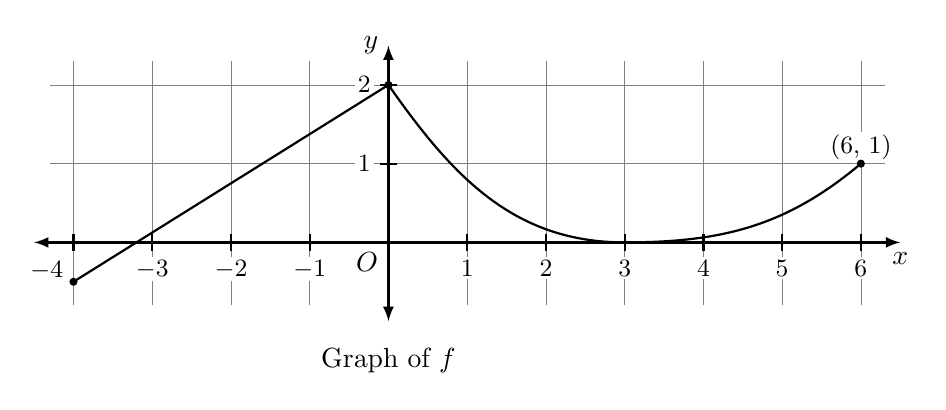
\begin{tikzpicture}[xscale=1,yscale=1,baseline=(current bounding box.north)]
        \draw[step=1,style=help lines,] (-4.3,-.8) grid (6.3,2.3);
        \draw[latex-latex, thick] (-4.5,0)-- (0,0) node [below left] {$O$}-- (6.5,0) node[below] {$x$};
        \draw[latex-latex, thick] (0,-1)--(0,2.5) node[left] {$y$};
        \foreach \x in {-3,-2,-1,1,2,3,4,5,6}
            \draw[thick] (\x,3pt) -- (\x,-3pt) node [below=.7mm,fill=white,inner sep=1pt] {\small$\x$};
        \draw[thick] (-4,3pt) -- (-4,-3pt) node [below left=.82mm,fill=white,inner sep=1pt] {\small$-4$};
        \foreach \y in {1,2}
            \draw[thick] (3pt,\y) -- (-3pt,\y) node [left=.7mm,fill=white,inner sep=1pt] {\small$\y$};
        
        \draw[-,thick] (-4,-.5) -- (0,2);
        \filldraw (-4,-.5) circle (1.25pt);
        \filldraw (0,2) circle (1.25pt);
        
        \draw[-,thick] (0,2) to [out=-55,in=180] (3,0);
        \draw[-,thick] (3,0) to[out=0,in=-140] (6,1) node [above,fill=white,inner sep=1pt] {\small$(6,\,1)$};
        \filldraw (6,1) circle (1.25pt);
        
        \node at (0,-1.5) {Graph of $f$};
        
    \end{tikzpicture}
\end{center}

\begin{questions}
    \setcounter{question}{2}
    \question A continuous function $f$ is defined on the closed interval $[-4,\,6]$. The graph of $f$ consists of a line segments and a curve that is tangent to the $x-$axis at $x=3$, as shown in the figure above. On the interval $0<x<6$, the function $f$ is twice differentiable, with $f''(x)>0$.\\
    \\
    Is there a value of $a$, with $-4\le a<6$, for which the Mean Value Theorem, applied on the interval $[a,\,6]$, guarantees a value $c$, with $a<c<6$, at which $f'(c)=\frac{1}{3}$? Justify your answer.
\end{questions}


\newpage
